\chapter{Methods}
\label{chapter4}

We propose a framework that synthesises planning and reinforcement learning which can overcome the inherent inaccuracies of models through hypothesising, through reasoning, changes to the model that would be most beneficial to the planner and then planning on this temporary model. The correctness of these changes is then realised through experience in the real environment, and the model is updated through generic model-learning.
We use the concept of \textit{optimism in the face of uncertainty}, we state that we are always almost in a state of uncertainty due to the inevitable inaccuracies of the model.
To enable the planner to make these hypotheses we equip it with additional actions which we denote Meta Actions.
\section{Meta Actions}
These actions do not cause the agent to act in the environment, and thus do not return any observation in terms of a new state and a reward, but rather cause changes directly to the model when called upon. An important factor and one of the main difficulties is deciding what Meta Actions should be exposed to the planner and when the planner should be able to invoke the Meta Actions. Therefore, we state three conditions which all must hold for a Meta Action to be invoked: a Meta Action must be admissible, feasible and reasonable.
\subsection{Admissible}
A Meta Action is admissible if applying it to the model leads to what seems like a better plan. If applying the Meta Action does not result in any benefit to the planner, but rather it negatively affects the planner, then it should not be called. In-fact due to the nature of planning, an inadmissible Meta Action would never be called.
\subsection{Feasible}
Feasibility is important, since it ensures that we don't contradict observations and don't infinitely hypothesise changes to the model. However, the definition of feasibility depends on the transition dynamics of the domain. In the deterministic case, a Meta Action is feasible if the state or state-action pair that it affects has not been previously observed, and changes to to that state or state-action pair have not been previously hypothesised.
For stochastic domains, the latter condition of deterministic domains is sufficient for a Meta Action to be feasible.
\subsection{Reasonable}
Often, the change to the model that would be of most benefit the planner, is to simply add a transition from the current state to the goal state. However, this is almost never going to be a change that is realised to be correct; and instead would lead to behaviour akin to taking a random-walk through the state space until the goal is reached and the Meta Actions have been exhausted. Hence, it's key that an additional constraint exists, that ensures Meta Actions which are called hypothesise reasonable changes to the model. We consider two key ways of determining reasonability: through embedding reasonable Meta Actions in the model by-hand and through learning Meta Actions directly from experience.

\section{The Framework}
Our framework consists of three distinct steps: planning (and hypothesising), execution and learning, which can be seen in Figure \ref{fig:framework}. These three steps occur during two phases. Within the planning phase, all three occur, however in the model-free phase, just execution and learning occur (and execution is driven by the current learned policy).

\subsection{Planning}
The choice of planner is largely irrelevant to the framework, we mostly consider heuristic search algorithms and planning by dynamic programming.
A temporary model is created. The planner then begins planning on this model, at each node (state), the planner considers both the actions and available Meta Actions - if a Meta Action is chosen, then that change is made to the temporary model and planning continues. The computed plan is then returned to the agent.
\subsection{Execution}
During the planning phase, the agent chooses actions by sampling a plan from the planner. During the model-free phase, the agent chooses actions from the learned policy. The agent then executes the action in the environment, observing its affects through its new state and the reward received.
\subsection{Learning}
There are two sections to the learning step: where the model is learned \cite{10.1145/122344.122377}, and  where the policy is learned. The model is learned, as a tabular maximum likelihood model. The policy is learned, by at each discrete time step  updating the maintained Q-values.

\section{Implementations}
The description of the framework above led to various implementations. The underlying concept of allowing the planner to hypothesise changes to the model is present throughout all of the frameworks, but the ways in which the planner decides which change is most beneficial differs, and in some places simplifications are offered for differing domains (deterministic vs stochastic). Each framework will be presented and highlighted here.
\subsection{RL-A* Meta, embedded reasonable actions (Deterministic)}
A simple model-based RL implementation; the agent explores by planning on the model, and learns the model as it does so.
Additionally, the planner is equipped with the following actions: RemoveObstacle, AddObstacle, DecreaseReward, IncreaseReward.
\subsection{RL-A* Meta, embedded reasonable actions, with short-term memory (Stochastic)}
A simple model-based RL implementation; the agent explores by planning on the model, and learns the model as it does so.
Additionally, the planner is equipped with the following actions: RemoveObstacle, AddObstacle, DecreaseReward, IncreaseReward. The planner approximates a deterministic model which it plans on. To allow for sufficient exploration, the agent has a short-term memory, encouraging it to try Meta Actions again, where it wouldn't be able to do so in the deterministic case.
\subsection{RL-VI Meta, embedded reasonable actions (Deterministic)}
A model-based RL implementation; the agent explores by planning on the model, and learns the model as it does so.
Additionally, the planner is equipped with the following actions: AddTransition, RemoveTransition, DecreaseReward, IncreaseReward.
\subsection{RL-VI Meta, embedded reasonable actions (Stochastic)}
A model-based RL implementation; the agent explores by planning on the model, and learns the model as it does so.
Additionally, the planner is equipped with the following actions: IncreaseTransitionProbability, DecreaseTransitionProbability, DecreaseReward, IncreaseReward.
\subsection{RL-VI Meta, with learning reasonable Meta Actions (Stochastic)}
A model-based RL implementation; the agent explores by planning on the model, and learns the model as it does so.
Additionally, the planner is equipped with the following actions: IncreaseTransitionProbability, DecreaseTransitionProbability, DecreaseReward, IncreaseReward. A key difference is that Meta Actions are learned and obtained through experience, rather than embedded by hand with the model.
% A typical approach of using planning for exploration would consist of sampling plans, following them, realising their correctness through experience, and updating the model accordingly. However, since we know that all models are inaccurate, it's very possible that the optimal policy may never be discovered in this way. In order to mitigate these inaccuracies, and enable the optimal policy to be discovered, we suggest various frameworks that enable the planner to hypothesise, through reasoning, changes to the model that would be beneficial; that would lead to a better policy than the current one. The correctness of these changes is then realised through experience. To enable the planner to hypothesise these changes, we equip it with additional actions which we denote \textbf{Meta Actions}, which when called upon do not cause the agent to act in the environment but rather affect the model. This is an optimistic approach, but not over-optimistic where the agent will hallucinate, since the changes are driven by reasoning. The concept of "optimism in the face of uncertainty" is present, except we are almost always in a state of uncertainty due to the inevitable inaccuracies of the model. Given sufficient planning steps, with this method the agent would explore all states that could possibly be on the optimal path, inducing an envelope that is explored between the start and goal state.

\begin{figure}[h!]
    \centering
    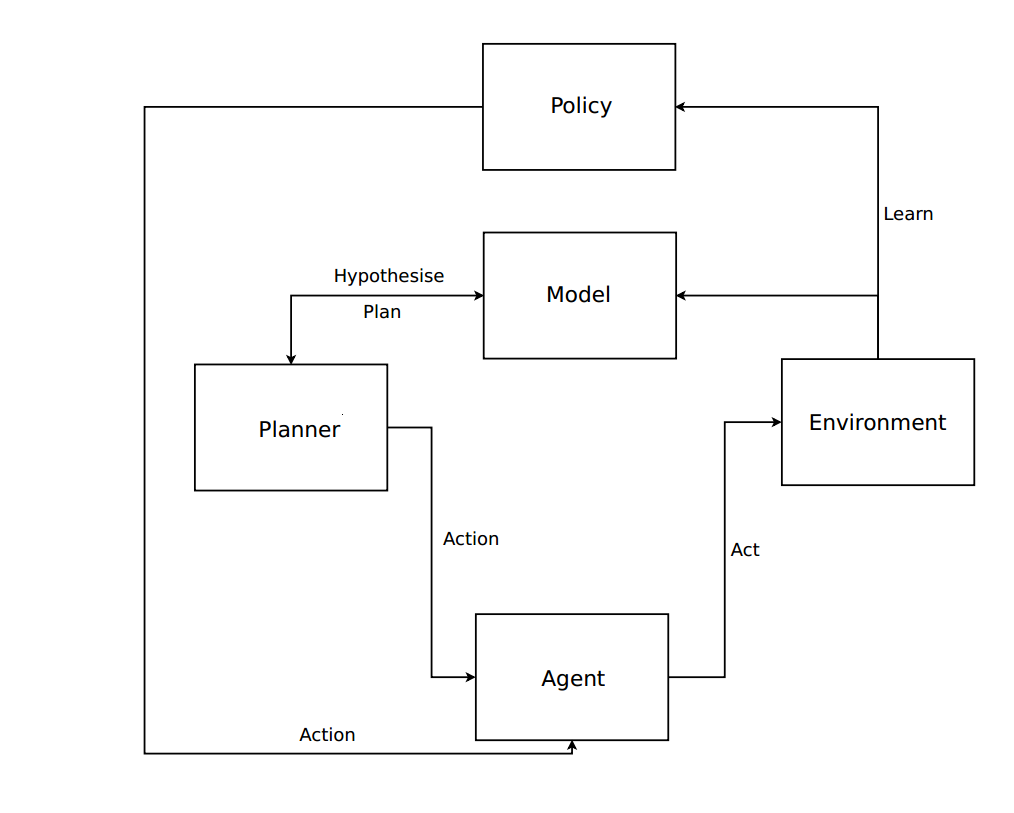
\includegraphics[max size={\textwidth}{\textheight}]{report/assets/diagram.png}
    \caption{Framework}
    \label{fig:framework}
\end{figure}

% \begin{figure}[h!]
%     \centering
%     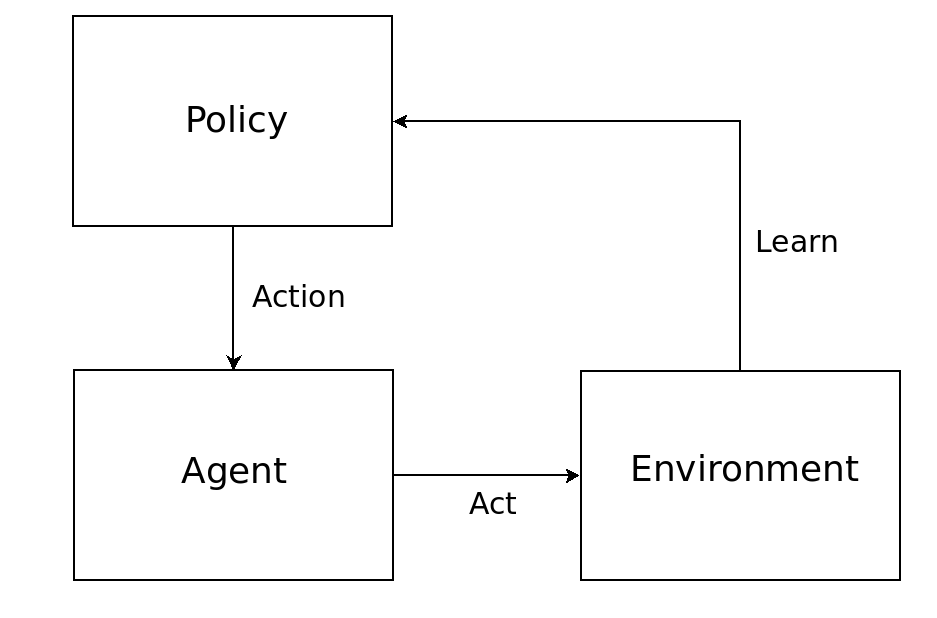
\includegraphics[max size={\textwidth}{\textheight}]{report/assets/rl_diagram.png}
%     \caption{Framework}
%     \label{fig:framework}
% \end{figure}

% % The core of this work is to follow a model-based RL approach, computing plans from a (inherently inaccurate) model to guide guide exploration, updating the model where necessary. What differentiates this from other works, highlighted in Chapter 2, is the additional actions exposed to the planner, that don't actually affect the environment, but rather the model; we deem these \textbf{Meta Actions}. The main idea is that the Planner can use these Meta Actions to hypothesise changes to the model that would be of most benefit, in this sense the approach is optimistic. The hypotheses are driven by reasoning.
% \section{Meta Actions}
% A Meta Action is an action which does not affect the environment in any way, thus the agent receives no observation or reward upon taking it, but rather it affects the model directly. For the Planner to suggest a Meta Action, it must be admissible, feasible and reasonable.
% \subsection{Admissable}
% A Meta Action is \textbf{admissable} if applying it to the model leads to what seems like a better plan. If applying the Meta Action does not result in any benefit to the planner, but rather it negatively affects the planner, then it should not be called.
% \subsection{Feasible}
% A Meta Action is \textbf{feasible} in the deterministic case if 1) the corresponding state or transition has not been previously observed 2) the Meta Action has not been previously called on the corresponding state or transition. For the stochastic case, a Meta Action is feasible if just 2 holds.
% \subsection{Reasonable}
% Since the change to the model that would most benefit the Planner is always to add a transition from the current state to the goal state, we need to add a constraint to what Meta Actions can be called, otherwise this results in random-walk-like behaviour.
% For instance, Meta Actions can be learned; when we realise differences between the environment and the model, we can learn this difference as a Meta Action. Otherwise, reasonability can be something that is embedded directly in the model. Thus, a Meta Action is \textbf{reasonable} if it has been directly learned through experience or it is embedded in the model by-hand.
% \section{Frameworks}

% \section{Link to Human Decision Making}
% \begin{itemize}
%     \item What if that road is busy today, etc.?
% \end{itemize}